\chapter{医院获得性肺炎和呼吸机相关性肺炎}

\section{前沿学术综述}

医院获得性肺炎(hospital-acquired
pneumonia,HAP)是患者住院期间发生的肺实质感染,指入院时既不存在,也不处于潜伏期的感染。根据美国国家医院获得性感染监测系统(national
nosocomial infection surveillance
system,NNIS)的资料,肺部感染已经超过泌尿系感染,成为最常见的医院获得性感染,医院获得性肺炎占所有医院获得性感染的27%。在美国,每年约有25万住院患者发生医院获得性肺炎,直接或间接导致3万名患者死亡,我国该病的患病率为1.3%~3.4%。重症医学科(ICU)医院获得性肺炎的患病率与其他住院患者相比增加10~20倍。医院获得性肺炎不仅使患者住院时间平均延长4~9天,也是导致医院获得性感染患者的主要死因。预防和控制医院获得性肺炎具有重要意义。

呼吸机相关性肺炎(ventilator-associated
pneumonia,VAP)是医院获得性肺炎的一种特殊类型,指机械通气48小时后发生的肺炎。根据患者人群不同,呼吸机相关性肺炎患病率在6%~52%不等。并发呼吸机相关性肺炎的患者重症医学科住院时间和总住院时间明显延长,住院费用明显增加。呼吸机相关性肺炎是患者病死率增高的独立危险因素,粗病死率达到30%~70%。

医院获得性肺炎可以由多种微生物病原体引起,常见的病原体包括需氧革兰阴性杆菌,如铜绿假单胞菌、大肠埃希菌、肺炎克雷伯菌和不动杆菌等;革兰阳性球菌,如葡萄球菌,特别是耐甲氧西林的金黄色葡萄球菌(methicillin-resistant
staphylococcus
aureus,MRSA)的感染逐年增多。此外,厌氧菌感染所致医院获得性肺炎在机械通气患者中较罕见。

导致呼吸机相关性肺炎的常见细菌包括革兰阴性杆菌和革兰阳性球菌,如铜绿假单胞菌、肺炎克雷伯杆菌、不动杆菌属、金黄色葡萄球菌(特别是MRSA)等,而且多药耐药(multidrug-resistant,MDR)细菌的比例在明显增高。近年来真菌感染也呈上升趋势。

\subsubsection{呼吸机相关性肺炎的诊断}

诊断呼吸机相关性肺炎基于两个方面:一是依据病史(机械通气48小时以上,有危险因素)、体格检查和X线胸片判断是否存在肺炎;二是明确感染的病原微生物。

目前诊断呼吸机相关性肺炎的金标准仍然是组织病理学有炎症反应和肺活组织培养微生物阳性,但此标准临床难以实现。临床诊断标准为X线胸片出现新的浸润阴影或原有浸润阴影扩大,同时具有下列三项中的两项或两项以上:①体温>38℃;②白细胞计数增高或降低;③脓性痰。此诊断标准的敏感性为69%,特异性为75%。临床肺部感染评分(clinical
pulmonary infection
score)有助于呼吸机相关性肺炎进行量化的诊断,主要从体温、血白细胞计数、痰液性状、X线胸片、氧合指数和半定量培养结果诊断呼吸机相关性肺炎,总分12分,一般以临床肺部感染评分>6分作为诊断标准,与金标准相比其敏感性为77%,特异性为42%,而简化的临床肺部感染评分更便于临床评估。2005年美国胸科协会(American
Thoracic Society,ATS)和美国感染病协会(Infectious Diseases Society of
America,IDSA)在医院获得性肺炎和呼吸机相关性肺炎指南中首次明确提出,临床肺部感染评分可以用于协助肺部感染的诊断和指导抗生素的调整
\protect\hyperlink{text00014.htmlux5cux23ch1-13}{\textsuperscript{{[}1{]}}}
。

微生物学诊断是指对下呼吸道分泌物进行定量培养,确定诊断阈值,超过阈值,可考虑诊断呼吸机相关性肺炎,低于阈值一般认为是定植或污染。其目的是判断何种微生物为致病菌,以及是否开始抗菌药物治疗、选择何种抗菌药物。保护性毛刷(protected
specimen brush)分泌物定量培养以>10\textsuperscript{3}
cfu/ml为诊断标准,支气管肺泡灌洗(bronchoalveolar
lavage)液定量培养以>10\textsuperscript{4}
cfu/ml为诊断标准,气管抽吸分泌物培养以>10\textsuperscript{6}
cfu/ml为诊断标准。特别强调在抗菌药物治疗前应留取标本,但不能因为需要留取标本或等待结果而延误抗菌药物治疗。

近年来部分研究显示,支气管肺泡灌洗液中的髓样细胞表达的可溶性触发受体I(sTREM-I)浓度的检测,也可作为早期诊断呼吸机相关性肺炎的手段,血浆降钙素原、支气管肺泡灌洗液中内毒素浓度检测,也可作为呼吸机相关性肺炎的筛选方法,阳性结果意味着需要更多的细菌学检测和及时经验性抗菌药物治疗,以及定期评价临床效果。

\subsubsection{呼吸机相关性肺炎的治疗}

重症感染及感染性休克导致患者病死率居高不下,一直在50%左右,为此2004年11个国际性组织在巴塞罗那联合推出了重症感染和感染性休克治疗指南,力争在全世界范围内通过教育和指南的推广,使重症感染和感染性休克的病死率在5年之内降低25%
\protect\hyperlink{text00014.htmlux5cux23ch2-13}{\textsuperscript{{[}2{]}}}
。而呼吸机相关性肺炎是目前重症医学科最常见的感染之一,早期合理的抗生素治疗和积极预防呼吸机相关性肺炎的发生非常重要。2004年加拿大危重病学会和加拿大危重病临床试验组联合组成专家委员会,以及2005年美国胸科医师协会和美国感染病协会先后制定了基于循证医学证据的医院获得性肺炎和呼吸机相关性肺炎方面的指南,对于医院获得性肺炎和呼吸机相关性肺炎的诊断和规范化治疗提出了许多建议
\protect\hyperlink{text00014.htmlux5cux23ch1-13}{\textsuperscript{{[}1{]}}}
、
\protect\hyperlink{text00014.htmlux5cux23ch3-13}{\textsuperscript{{[}3{]}}}
、
\protect\hyperlink{text00014.htmlux5cux23ch4-13}{\textsuperscript{{[}4{]}}}
。呼吸机相关性肺炎的治疗原则主要是根据病原菌是否存在多药耐药(MDR)危险性和肺炎发生的时间,结合本单位具体情况,早期及时应用合适、足量的抗菌药物,并根据微生物学涂片结果、培养和患者的临床治疗反应做相应调整。

近年来,在医院获得性肺炎和呼吸机相关性肺炎防治上,强调针对感染危险因素应用多种非抗生素抗感染策略集束化预防。根据循证医学证据,强烈推荐将半卧位、洗手、持续声门下吸引应用于机械通气患者呼吸机相关性肺炎的预防
\protect\hyperlink{text00014.htmlux5cux23ch5-13}{\textsuperscript{{[}5{]}}}
。近来研究显示早期经皮胃造瘘和洗必泰口腔护理也可以降低呼吸机相关性肺炎的发生率
\protect\hyperlink{text00014.htmlux5cux23ch6-13}{\textsuperscript{{[}6{]}}}
\textsuperscript{,}
\protect\hyperlink{text00014.htmlux5cux23ch7-13}{\textsuperscript{{[}7{]}}}
。鉴于热湿交换器和封闭式吸痰在对于降低呼吸机相关性肺炎发生率方面无明确的临床循证医学证据支持
\protect\hyperlink{text00014.htmlux5cux23ch8-13}{\textsuperscript{{[}8{]}}}
\textsuperscript{~}
\protect\hyperlink{text00014.htmlux5cux23ch10-13}{\textsuperscript{{[}10{]}}}
,目前并不推荐常规应用热湿交换器和封闭式吸痰。

\section{临床问题}

\subsection{流行病学与发病机制}

\subsubsection{何谓医院获得性肺炎?}

医院获得性肺炎又称医院内肺炎(nosocomial
pneumonia),指患者入院48小时后发生的肺炎,入院时既不存在、也不处于感染潜伏期。2005年美国胸科协会和美国感染病协会制定的医院获得性肺炎指南中,医院获得性肺炎也包括了两种特殊的类型:呼吸机相关性肺炎和卫生保健相关性肺炎(healthcare-associated
pneumonia),后者包括下列肺炎病人:①最近90天内住院超过2天以上者;②居住在护理之家或长期护理机构者;③接受透析治疗者;④接受家庭输液治疗(抗生素)者;⑤接受过伤口处理者;⑥家庭成员携带多药耐药菌者。

目前认为,在医院获得性感染(包括医院获得性肺炎、血源性感染、泌尿系感染、外科伤口感染、导管相关性感染等)所致的死亡中,医院获得性肺炎是主要死因。

\subsubsection{医院获得性肺炎病原学如何分布?}

医院获得性肺炎可以由多种微生物病原体引起,医院获得性肺炎常见的病原体包括需氧革兰阴性杆菌,如铜绿假单胞菌、大肠埃希菌、肺炎克雷伯菌和不动杆菌等;革兰阳性球菌,如葡萄球菌,特别是耐甲氧西林的金黄色葡萄球菌的感染逐年增多,有研究显示,美国重症医学科中葡萄球菌所致的感染,耐甲氧西林的金黄色葡萄球菌超过50%。在患者免疫力正常的情况下较少发生病毒和真菌的感染。在免疫功能低下的人群,例如器官移植后患者、艾滋病毒感染者以及糖尿病、中性粒细胞减少、潜在肺病和终末期肾脏疾病患者容易发生病毒与真菌感染。此外,厌氧菌感染所致医院获得性肺炎在机械通气患者中较罕见。我国医院内病原菌耐药监测(nosocomial
pathogen resistance
surveillance,NPRS)在1994~2002年的8年间,共分离到12821株革兰阴性杆菌,最常见的是铜绿假单胞菌、大肠埃希菌、克雷伯菌属、不动杆菌属、肠杆菌属、嗜麦芽窄食单胞菌,呼吸道标本中最常见的是铜绿假单胞菌、肺炎克雷伯菌和鲍曼不动杆菌。

早发性(指入院后48小时到5天内发生的)医院获得性肺炎多是由敏感菌,如肺炎链球菌、流感嗜血杆菌、甲氧西林敏感金黄色葡萄球菌(methicillin-sensitive
staphylococcus
aureus,MSSA)和敏感的肠道革兰阴性杆菌(如大肠杆菌、肺炎克雷伯杆菌、变形杆菌和黏质沙雷杆菌)引起的感染。

晚发性(指入院时间≥5天)医院获得性肺炎则很可能是多药耐药(MDR)细菌所致,包括铜绿假单胞菌、产超广谱β-内酰胺酶(extended
broad-spectrum
β-lactamase,ESBL)的肺炎克雷伯杆菌和鲍曼不动杆菌、耐药肠道细菌属、嗜麦芽窄食假单胞菌,以及耐甲氧西林的金黄色葡萄球菌等,免疫抑制患者还需考虑嗜肺军团菌感染可能。

当然,早发性医院获得性肺炎患者如果近期接受过抗生素治疗或在健康护理院住院,也存在多药耐药病原菌定植和感染的危险性,患者病死率明显增高。多药耐药病原菌的流行情况依患者的基础疾病状态、所在地区和医院以及重症医学科的种类而有所不同。

\subsubsection{多药耐药病原菌引起医院获得性肺炎的危险因素有哪些?}

引起医院获得性肺炎的病原菌是否为多药耐药细菌,需考虑是否存在以下危险因素:①先前90天内接受过抗菌药物治疗;②本次住院5天以上;③社区或医院特殊病房中存在高发细菌耐药;④存在卫生保健相关性肺炎危险因素------最近90天内住院2天以上、居住在护理之家或扩大护理机构、家庭静脉治疗(包括抗菌药物)、30天内进行过慢性透析治疗、家庭伤口护理;家庭成员携带多药耐药菌;⑤存在免疫抑制性疾病和(或)在使用免疫抑制剂治疗。

\subsubsection{常见的多药耐药革兰阴性杆菌耐药现状如何?}

常见的多药耐药革兰阴性杆菌耐药主要有铜绿假单胞菌、不动杆菌属(鲍曼不动杆菌等)、产超广谱β-内酰胺酶的革兰阴性菌、产诱导酶细菌、嗜麦芽窄食单胞菌等。

(1)铜绿假单胞菌 是医院获得性肺炎中最常见的多药耐药病原菌。国内外资料表明,铜绿假单胞菌对β-内酰胺类、碳青霉烯类、氨基糖苷类、氟喹诺酮类耐药率呈增加趋势。我国医院内病原菌耐药监测显示,1994~2002年间,铜绿假单胞菌对亚胺培南和头孢他啶的敏感率已分别从1994年的96%、92%降至2001年的75%、79%,目前敏感率较高为阿米卡星和哌拉西林/三唑巴坦(分别为83%、81%),但阿米卡星由于耳、肾毒性造成应用范围受限。2005年来自日本60个医学中心分离的细菌菌株耐药监测显示,铜绿假单胞菌对头孢哌酮/舒巴坦的耐药率为12.5%,对泰能的耐药率高达30.8%。铜绿假单胞菌耐药机制复杂,有研究表明,外膜孔蛋白D(outer
membrane porin channel
D,OprD)的表达减少或丢失是导致铜绿假单胞菌对亚胺培南耐药的重要机制之一。

(2)不动杆菌属(鲍曼不动杆菌等) 对大多数抗菌药物,包括氨基糖苷类、喹诺酮类和广谱的β内酰胺类抗菌药物都耐药。不同菌种对抗菌药物的敏感性不同,其中鲍曼不动杆菌耐药最为严重,容易获得优势生长,其特点是定植菌多于感染菌,在健康人群中其定植率>40%,而在住院患者中定植率高达75%。亚胺培南对不动杆菌活性最高,超过85%的菌株对碳青酶烯类敏感,但由于IMP型或OXA型碳青霉烯酶的产生使细菌耐药性增加。在2005年美国胸科协会和美国感染病协会的医院获得性肺炎指南中,推荐用多黏菌素E治疗碳青霉烯耐药的不动杆菌感染。

(3)产超广谱β-内酰胺酶的革兰阴性菌 肺炎克雷伯菌和大肠埃希菌是常见的产超广谱β-内酰胺酶的细菌。质粒介导的超广谱β-内酰胺酶是由于β内酰胺酶的1~4个氨基酸突变而造成的,能够水解β内酰胺类抗生素和氨曲南,造成细菌对上述药物耐药,同时对其他大多数抗菌药物如氟喹诺酮类和氨基糖苷类耐药。超广谱β-内酰胺酶可以被克拉维酸、舒巴坦和三唑巴坦所抑制。我国流行的超广谱β-内酰胺酶亚型以CTX-M型为主,而在欧美各国以TEM型常见。

(4)产诱导酶细菌 诱导酶是染色体介导的头孢菌素酶,称Ⅰ类酶,又称诱导酶。阴沟肠杆菌、弗劳地枸橼酸杆菌、粘质沙雷菌和铜绿假单胞菌中可分离到此类酶。诱导酶不能被酶抑制剂所抑制,因此产诱导酶的细菌对所有的β内酰胺类/酶抑制剂复合制剂及头霉素均耐药,并且常常对氨基糖苷类和喹诺酮类耐药。治疗药物仅能选择碳青霉烯类和第四代头孢菌素。

(5)嗜麦芽窄食单胞菌 该菌是一种非发酵菌。我国医院内病原菌耐药监测显示,1994~2002年间分离的12821株革兰阴性菌中,嗜麦芽窄食单胞菌居全部标本的第7位,在呼吸道标本中居第6位。该菌天然产生金属酶,可以水解碳青霉烯类,故其对亚胺培南和许多β内酰胺类抗生素天然耐药。临床上复方磺胺嘧啶、米诺环素、左氧氟沙星和替卡西林/克拉维酸有时可以作为药物治疗的选择之一。

\subsubsection{如何评价多药耐药革兰阳性球菌的耐药现状?}

近年来多药耐药革兰阳性球菌逐渐增多,常见的病原菌及耐药现状如下。

(1)耐青霉素肺炎链球菌(penicillin-resistant streptococcus
pneumoniae,PRSP) 1965年美国首次报道肺炎链球菌对青霉素耐药,近年来耐药菌株逐渐增多,国外达30%~50%,国内王辉等报告显示约22.7%,对头孢呋新、大剂量阿莫西林、阿莫西林/棒酸、头孢噻肟、头孢曲松或氟喹诺酮尚敏感,但对红霉素、克林霉素、磺胺等药物多耐药。对以上药物都耐药时只能使用万古霉素或替考拉宁治疗。

(2)耐甲氧西林金黄色葡萄球菌及表皮葡萄球菌 该耐药菌已出现40余年,近年来直线上升。美国1975年耐药率仅2.4%,20世纪末达25%,近年来已达50%。在我国情况更为严重,上世纪末已达50%,本世纪以来不少三甲医院已达80%以上。耐甲氧西林的金黄色葡萄球菌已经成为院内感染的主要细菌之一,它们对除万古霉素和替考拉宁以外的常用抗生素均耐药。更可怕的是,国外出现了对万古霉素中介、甚至耐药的金黄色葡萄球菌,前者多选用万古霉素加利福平、阿米卡星等,耐万古霉素的金黄色葡萄球菌只有依靠更新的抗生素,如利奈唑胺(linezolid)、奎奴普丁/达福普汀(quinupristin/dalfopristin)。所幸国内尚未发现耐万古霉素的耐甲氧西林的金黄色葡萄球菌菌株。

(3)耐药肠球菌 包括粪肠球菌、屎肠球菌。耐药肠球菌不但对一般抗球菌药及广谱抗生素耐药,而且对特异性、很少耐药的万古霉素也耐药,即耐万古霉素肠球菌,1988年英国首次发现。国外报道发生率为7.9%~20%,国内10%~12.5%。治疗上根据药敏选用敏感抗生素,如替考拉宁或氨基糖苷类,体外研究显示新药利奈唑胺、达福普丁/奎奴普汀可用于耐万古霉素的肠球菌治疗。

\subsubsection{有哪些危险因素可以导致医院获得性肺炎的发生?}

医院获得性肺炎的危险因素可分为患者相关因素、感染控制相关因素和治疗相关因素等3类。

(1)患者相关因素 患者相关因素是医院获得性肺炎发生的基本条件。严重的急或慢性疾病、昏迷、营养不良、长期住院、低血压、代谢性酸中毒、吸烟以及同时患有多种疾病(包括中枢神经系统功能障碍、慢性阻塞性肺病、糖尿病、酗酒、氮质血症和呼吸功能衰竭等),均可通过影响患者的自身防御功能,导致细菌定植和感染。由于老年人多数患有多种疾病,因而发生肺炎的危险性增加,此外衰老导致的免疫功能下降也起一定的作用。

(2)感染控制相关因素 致病菌暴露或致病菌定植是医院获得性肺炎发生的必要条件。住院患者通常有很多机会接触大量细菌。细菌可通过医务人员的手在不同患者间传播。常见的原因包括接触不同患者之间不洗手或不更换手套,或使用污染的呼吸治疗设备等。胃肠道通常被认为是肠道革兰阴性杆菌的储存库,误吸可导致大量致病菌进入呼吸道导致感染。

(3)治疗相关因素 治疗相关的因素也参与了医院获得性肺炎的发生。镇静药抑制中枢神经系统功能,增加误吸发生率;糖皮质激素和细胞毒药物影响机体防御机制;长时间外科手术,特别是胸腹联合手术,改变呼吸道纤毛功能和细胞免疫,增加口咽部细菌的定植和肺炎的发生率。此外,长期不适当的抗生素治疗、制酸药的应用等治疗措施,也能增加患者接触大量细菌的机会。接受呼吸治疗患者的医院获得性肺炎发生率(7.7%),明显高于不接受呼吸治疗者(0.3%)。气管插管、气管切开或机械通气的患者发生肺部感染的危险性增加4~66倍。气管插管能影响下呼吸道的纤毛运动,妨碍分泌物的排出,同时破坏上皮细胞表面,使得细菌容易与下呼吸道表面结合。

按内源性和外源性因素分类,医院获得性肺炎发生的主要危险因素见表\ref{tab8-1}。

\begin{table}[htbp]
\centering
\caption{医院获得性肺炎的内源性和外源性危险因素}
\label{tab8-1}
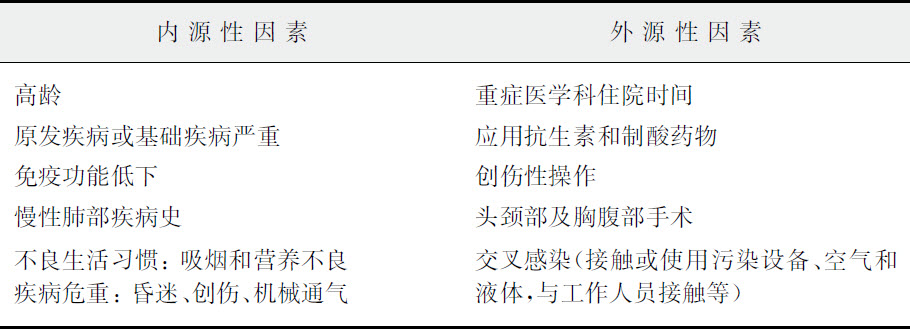
\includegraphics{./images/Image00059.jpg}
\end{table}

\subsubsection{医院获得性肺炎的发病机制是什么?}

医院获得性肺炎的主要发病机制包括口咽部微生物和(或)含微生物的胃内容物的误吸、吸入含有细菌的微粒或远处感染灶的血行播散。

(1)误吸口咽部微生物和(或)含微生物的胃内容物的误吸是医院获得性肺炎最重要的致病因素。

大多数细菌性肺炎,无论是否为医院获得性,其致病菌多为口咽部的细菌。约有10%的健康人口咽部有革兰阴性杆菌的定植。而住院和应激状态下细菌定植可显著增加。30%~40%的普通患者入院后48小时内即有细菌的定植,而危重患者则达70%~75%。革兰阴性杆菌在口咽部或气管支气管的定植是通过与宿主的上皮细胞粘附开始的。许多因素可以影响粘附,如细菌因素(鞭毛、纤毛、荚膜或产生弹力酶等)、宿主细胞因素(表面蛋白和多糖)以及环境因素(pH值和呼吸道分泌物中的粘蛋白)。尽管确切的作用机制尚不明确,但已有研究表明某些物质如纤维连接素能抑制革兰阴性杆菌与宿主细胞的粘附。相反,营养不良、危重病或术后等情况,均可促进细菌粘附,导致细菌定植明显增加。口咽部定植的细菌误吸是医院获得性肺炎发病的必要条件。Huxley等人用同位素示踪法发现,45%的正常人在熟睡时存在误吸。而那些吞咽困难、神志不清、气管插管和(或)机械通气、胃肠道疾患和术后的患者,则更容易发生误吸(70%)。所以,对危重患者而言,误吸是普遍存在的现象,不同的是误吸的量或程度的差异。即使带有套囊的气管切开管也不能防止误吸,研究显示,低容量高压气囊和高容量低压气囊分别有80%和15%的患者发生误吸。口咽部定植的细菌发生误吸后,由于肺部防御机制的障碍(如糖皮质激素、抗生素、氮质血症、酸中毒、经气管吸痰、酗酒或糖尿病等)将引起医院获得性肺炎。

对于机械通气患者,胃是口咽部革兰阴性定植菌的主要来源。健康人胃内pH值低于2,基本处于无菌状态。但当胃内pH值高于4时,微生物即在胃内大量繁殖,在高龄、胃酸缺乏、肠梗阻或上消化道疾患,以及接受胃肠营养、抗酸药或H\textsubscript{2}
受体拮抗剂治疗的患者尤为常见。研究表明,胃内pH值为1.0时,胃液中无细菌生长;而当pH值增加到6.0时,胃液内菌落增至10\textsuperscript{7}
cfu/ml以上。应用西米替丁治疗已被证实是医院获得性肺炎的危险因素之一。因此,应激性溃疡的预防也有其副作用。硫醣铝在保护胃黏膜的同时并不降低胃内pH值。有研究表明,与抗酸药或H\textsubscript{2}
受体拮抗剂相比,硫醣铝能够减少医院获得性肺炎的发生。应用局部或胃肠道不吸收抗生素进行选择性胃肠道去污染(selective
digestive
decontamination,SDD),有可能减少需氧革兰阴性杆菌引起的呼吸道感染,但现有资料不足以推荐选择性胃肠道去污染常规应用于所有患者。

(2)吸入含有细菌的微粒 细菌进入下呼吸道的另一种方式是通过吸入被呼吸治疗或麻醉设备污染的空气。呼吸机雾化装置能通过超声雾化作用产生大量<4μm的微粒,一旦受到污染,其产生的微粒可含有高浓度的细菌,从而进入下呼吸道深部。

(3)远处感染灶的血行播散 细菌性肺炎也可能是远处感染灶通过血行播散所致,这种情况较为少见。动物实验显示,细菌可从胃肠道经由上皮黏膜进入肠系膜淋巴结,最终至肺(细菌移位)。胃肠道细菌移位导致医院获得性肺炎可能发生于免疫抑制、肿瘤和烧伤等患者。

\subsection{临床诊断}

\subsubsection{呼吸机相关性肺炎的诊断标准是什么?}

目前呼吸机相关性肺炎的诊断标准尚不统一。常用的美国国家医院感染监测系统关于呼吸机相关性肺炎的诊断标准包含X线胸片、临床和微生物几个方面(表\ref{tab8-2})。

\begin{table}[htbp]
\centering
\caption{美国国家医院感染监测系统关于呼吸机相关性肺炎的诊断标准}
\label{tab8-2}
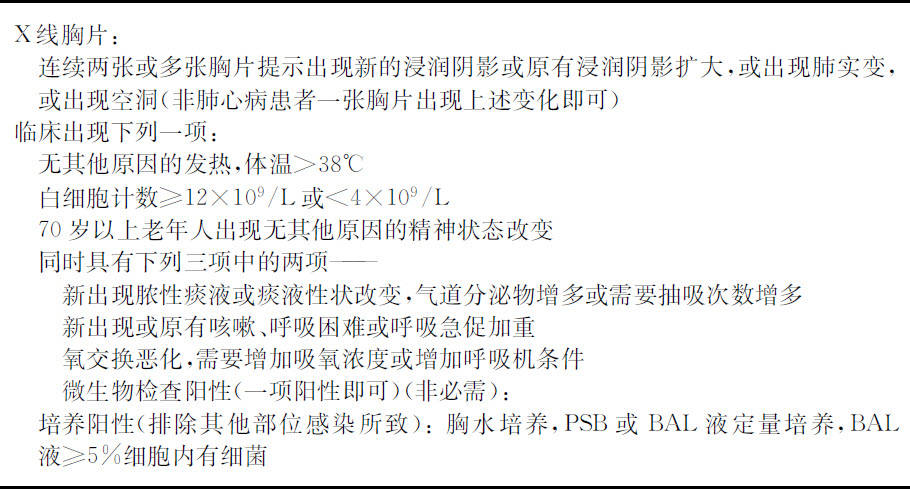
\includegraphics{./images/Image00060.jpg}
\end{table}

\subsubsection{呼吸机相关性肺炎的临床诊断标准应用时有哪些注意事项?}

常用的呼吸机相关性肺炎临床诊断标准包括X线胸片上新出现浸润阴影或原有浸润阴影扩大,同时具有下列三项中的两项及以上:①体温>38℃;②白细胞计数增高或降低;③脓性痰。临床操作比较简便,但在具体实践中因无统一的标准和主观差异导致诊断的敏感性和特异性差异很大。

诊断标准强调X线胸片和临床的表现,但二者均不特异。根据体温、白细胞计数和痰的性质很难区分肺部感染和化脓性气管支气管炎。在机械通气的患者,由于急性呼吸窘迫综合征(ARDS)和其他弥漫性肺损伤,临床表现更缺乏特异性。研究表明,肺炎在ARDS患者的急性期非常普遍却常常不被认识。另外,危重患者肺部出现浸润影应注意同肺不张、ARDS、肺栓塞、氧中毒及心力衰竭等进行鉴别。

此外,没有任何临床表现的患者不代表没有肺炎。尸检研究常常发现没有肺炎临床表现的患者存在肺炎而这部分患者并未接受抗菌药物治疗,这提示临床的主观印象可能并不准确,呼吸机相关性肺炎的临床诊断标准(X线胸片异常结合临床表现)可以进行呼吸机相关性肺炎的初筛,但是由于特异性较差,需要采用其他方法(如下呼吸道分泌物的涂片、培养等确定致病菌)和临床肺部感染评分等协助诊断。

\subsubsection{呼吸机相关性肺炎有哪些病原学诊断方法?}

呼吸机相关性肺炎病原学诊断方法包括:①气管内吸引;②经纤维支气管镜方法采样,如支气管肺泡灌洗、保护性毛刷;③血培养和胸腔积液培养;④经纤维支气管镜肺活检和开胸肺活检;⑤尸检;⑥其他,如盲法保护性毛刷、盲法支气管肺泡灌洗等
\protect\hyperlink{text00014.htmlux5cux23ch11-13}{\textsuperscript{{[}11{]}}}
。尤以前三种方法临床上常用。

对于机械通气患者,利用气管内吸引留取标本进行涂片和培养,操作简单,在床旁即可操作,无需复杂的培训。若每个低倍视野下的多形核白细胞不少于25个,上皮细胞不多于10个,尤其当镜下发现大量形态一致的致病菌时,提示下呼吸道存在细菌感染。涂片的结果往往可以为临床更早提供病原学参考。气道内吸引标本培养>10\textsuperscript{6}
cfu/ml,则诊断呼吸机相关性肺炎的敏感性为38%~91%,特异性为59%~92%。但对于感染、定植和污染的鉴别有时仍很困难。

通过支气管镜进行支气管肺泡灌洗和保护性毛刷检查,可直接从下呼吸道取材,而不易被上呼吸道或口腔分泌物污染。当支气管肺泡灌洗液培养结果>10\textsuperscript{4}
cfu/ml、保护性毛刷标本培养结果>10\textsuperscript{3}
cfu/ml时可诊断为呼吸机相关性肺炎。经支气管镜采样诊断有较高的特异性,但在近期使用或更换过抗生素的情况下有可能出现假阴性结果。

血培养对诊断和预后评价有一定价值,建议同时进行检查,但阳性率仅6%。选择合适的采血时间、足够的血量和次数可能有助于提高阳性率。

\subsubsection{保护性毛刷对诊断呼吸机相关性肺炎的意义如何?}

1979年保护性毛刷开始在临床应用,最初用于肺炎诊断,也可用于呼吸机相关性肺炎的诊断。通常采用10\textsuperscript{3}
cfu/ml作为临界值(大致相当于感染部位的密度为10\textsuperscript{6}
cfu/ml)来区分下呼吸道感染与口咽部或气管细菌定植。保护性毛刷的敏感性为40%~100%(多数报道在60%~90%),特异性50%~80%。

然而,保护性毛刷也存在下列问题:①口咽部细菌的污染导致假阳性结果;②应用抗菌药的患者细菌数可低于10\textsuperscript{3}
cfu/ml;③支气管炎患者因细菌负荷较少,保护性毛刷很少高于10\textsuperscript{3}
cfu/ml;④对于保护性毛刷的重复性研究显示,在25%的致病菌和多至40%的患者中,多次保护性毛刷的结果并不一致;⑤培养结果需在24~48小时后才能得到;⑥对临界值的确定仍存在疑问。

相当多的研究对保护性毛刷和其他有创诊断方法(多为支气管肺泡灌洗)的准确性进行了比较,支气管肺泡灌洗敏感性较高,而保护性毛刷特异性较高,但总体结果并未发现其中哪种方法更为优越。

总之,在诊断呼吸机相关性肺炎方面,保护性毛刷的特异性超过其敏感性,有条件或诊断困难时可以使用。

\subsubsection{如何评价支气管肺泡灌洗对诊断呼吸机相关性肺炎的意义?}

支气管肺泡灌洗是指在纤维支气管镜直接插至下呼吸道采集炎症部位标本,以及对支气管以下肺段或亚肺段水平反复以无菌生理盐水灌洗、回收,并对其进行一系列检测和分析。

1988年以后,支气管肺泡灌洗开始用于呼吸机相关性肺炎的诊断。与保护性肺毛刷相比,支气管肺泡灌洗更为简便和安全,而且能够对更大范围的肺组织留取标本,目前多以10\textsuperscript{4}
cfu/ml作为诊断呼吸机相关性肺炎的临界值。另外,Johanson等人根据狒狒的支气管肺泡灌洗标本培养结果中的细菌菌落计数,定义细菌指数(bacterial
index,BI),并发现支气管肺泡灌洗的BI值与肺组织培养后菌落计数结果呈正相关,从而提出以细菌指数>5.0区分肺部感染和细菌定植。对支气管肺泡灌洗标本进行定量培养并计算含有致病菌的细胞百分比(以25%以上的细胞中含有细菌作为诊断分界线),发现支气管肺泡灌洗的诊断敏感性显著高于保护性毛刷。可见,支气管肺泡灌洗能够在定量和定性两个方面反映肺内细菌感染的情况。

支气管肺泡灌洗诊断呼吸机相关性肺炎的敏感性差异很大,平均为(73±18)%,特异性平均为(82±19)%。造成差异的原因包括既往使用抗菌药、研究人群以及采取的参照诊断标准等。值得注意的是,计算的敏感性与定量培养的临界值密切相关。另外,支气管肺泡灌洗的临床应用仍存在一些问题,如诊断标准尚未完全统一,操作步骤尚未标准化,与保护性毛刷结果的一致性较差等,尚有待于进一步研究解决。

近来主张将支气管肺泡灌洗与保护性毛刷相结合,从而使诊断的敏感性和特异性显著提高。

\subsubsection{临床肺部感染评分在呼吸机相关性肺炎诊断中的意义如何?}

临床肺部感染评分是一项综合了临床、影像学和微生物学标准等来评估感染严重程度,协助指导抗菌药物调整的评分系统,对诊断、治疗和评价肺炎患者有一定的意义。

临床肺部感染评分指标包括体温、白细胞计数、气管分泌物、氧合情况、X线胸片和气管吸取物培养,最高评分为12分(表\ref{tab8-3})\footnote{*总分为12分,机械通气情况下临床肺部感染评分>6分提示存在呼吸机相关性肺炎。}。接受机械通气的重症医学科患者临床肺部感染评分>6分即可被诊断为呼吸机相关性肺炎,其与支气管肺泡灌洗诊断有较好的相关性,有研究表明其相关性为0.84。鉴于临床肺部感染评分标准中气道分泌物半定量分析在临床实际工作中有时应用困难,Luma
\protect\hyperlink{text00014.htmlux5cux23ch12-13}{\textsuperscript{{[}12{]}}}
在研究中提到简化的临床肺部感染评分,更便于临床操作,其指标包括体温、血白细胞、气道分泌物、氧合指数和X线胸片,共计10分,≥5分可诊断呼吸机相关性肺炎,联合痰涂片可提高诊断的准确性(表\ref{tab8-4})。\footnote{*
总分为10分,机械通气情况下临床肺部感染评分≥5分提示存在呼吸机相关性肺炎。}

\begin{table}[htbp]
\centering
\caption{诊断呼吸机相关性肺炎的临床肺部感染评分标准\textsuperscript{*}}
\label{tab8-3}
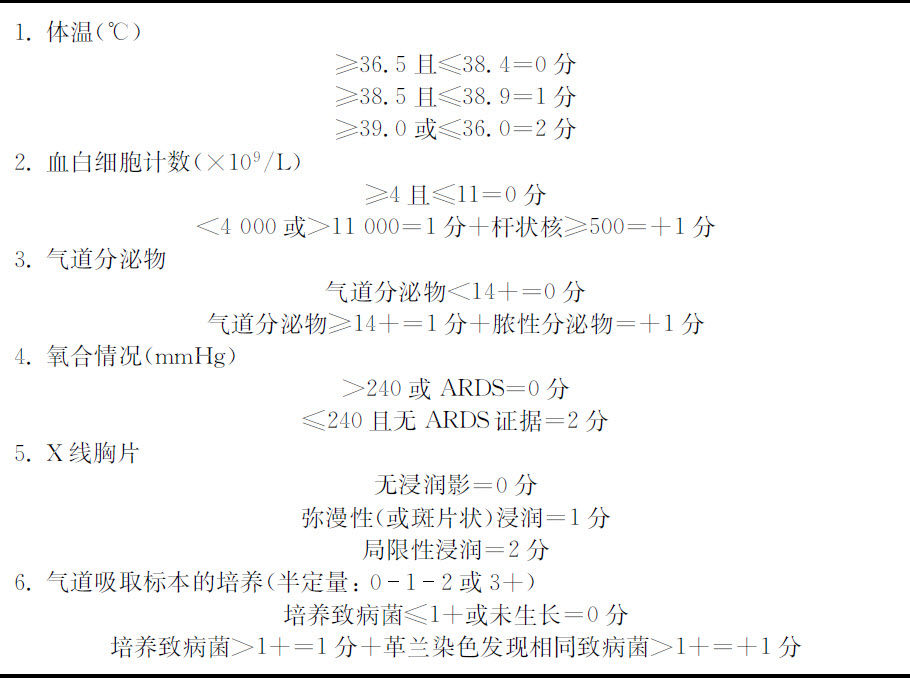
\includegraphics{./images/Image00061.jpg}
\end{table}

\begin{table}[htbp]
\centering
\caption{诊断呼吸机相关性肺炎的简化临床肺部感染评分标准\textsuperscript{*}}
\label{tab8-4}
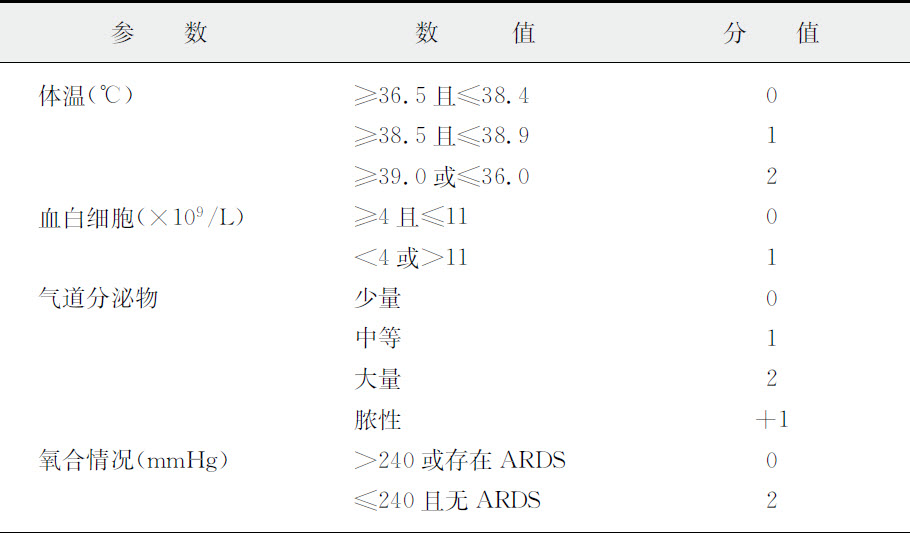
\includegraphics{./images/Image00062.jpg}
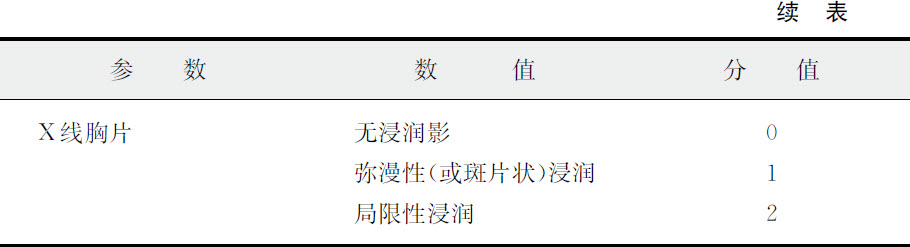
\includegraphics{./images/Image00063.jpg}
\end{table}

持续评价临床肺部感染评分可评估呼吸机相关性肺炎患者的临床转归。一项对427例接受机械通气>72小时患者的研究表明,与发病前3天相比,所有呼吸机相关性肺炎患者发病时的临床肺部感染评分均显著升高。存活组患者呼吸机相关性肺炎发病前3天及发病时的临床肺部感染评分与死亡组相似,但在发病后的第3、5及7天,存活组的临床肺部感染评分显著低于死亡组。氧合指数与转归的相关性最好,在治疗3天后,适当抗生素治疗组的氧合指数>250mmHg,不适当治疗组则持续下降。不过,在近期的研究中,分别计算第1、3天的临床肺部感染评分变化,与呼吸机相关性肺炎患者的病死率并无相关性
\protect\hyperlink{text00014.htmlux5cux23ch13-13}{\textsuperscript{{[}13{]}}}
。

在2005年美国胸科协会(ATS)和美国感染病协会(IDSA)指南中建议应用临床肺部感染评分作为提高临床诊断特异性的工具,协助呼吸机相关性肺炎的诊断和指导抗生素的调整,在保证疗效的前提下尽量缩短抗菌药物的疗程。

\subsubsection{如何评价髓样细胞表达的可溶性触发受体I在呼吸机相关性肺炎诊断中的意义?}

髓样细胞表达的可溶性触发受体I属于免疫球蛋白家族,在中性粒细胞、成熟单核细胞和巨噬细胞表面表达。其能够协同Toll样受体增强微生物感染所致的炎症反应,但对于非感染性免疫复合物所致的炎症反应无促进作用。有研究显示,通过检测支气管肺泡灌洗(BAL)液中的髓样细胞表达的可溶性触发受体I来诊断细菌性呼吸机相关性肺炎,比临床肺部感染评分和降钙素原更准确。应用髓样细胞表达的可溶性触发受体I判断是否存在肺炎的受试者工作特征曲线下面积达0.93,多因素逻辑回归分析提示髓样细胞表达的可溶性触发受体I是判断是否存在肺炎的最重要独立因素,比值比高达41.5。以肺泡灌洗液中髓样细胞表达的可溶性触发受体I浓度200pg/ml作为诊断标准,其灵敏度74%,特异度88%。

因此,检测肺泡灌洗液中的髓样细胞表达的可溶性触发受体I浓度可作为诊断肺炎尤其是诊断呼吸机相关性肺炎的重要手段之一。

\subsubsection{降钙素原是否可以用于呼吸机相关性肺炎的诊断?}

降钙素原是由116个氨基酸组成的无活性的降钙素前体,由甲状腺C细胞合成。健康成人血液中浓度极低,低于0.1mg/L。降钙素原在全身感染中的病理生理学作用机制尚不清楚。细菌感染患者降钙素原血浆浓度增高,可能是细菌毒素直接作用结果,也可能是致炎因子介导的间接反应。实验研究认为降钙素原可能是全身感染导致炎症因子产生过程中的中间产物。目前认为血浆降钙素原浓度高于0.25mg/L,可作为诊断呼吸机相关性肺炎和开始抗菌药物治疗的辅助指标。

\subsubsection{如何诊断重症医院获得性肺炎?}

除确定医院获得性肺炎诊断外,认识其严重程度对于经验性选择抗菌药物,进行支持性治疗以及估计患者预后也非常重要。美国胸科协会提出了重症医院获得性肺炎的诊断标准(表\ref{tab8-5})。

\begin{table}[htbp]
\centering
\caption{重症医院获得性肺炎的诊断标准}
\label{tab8-5}
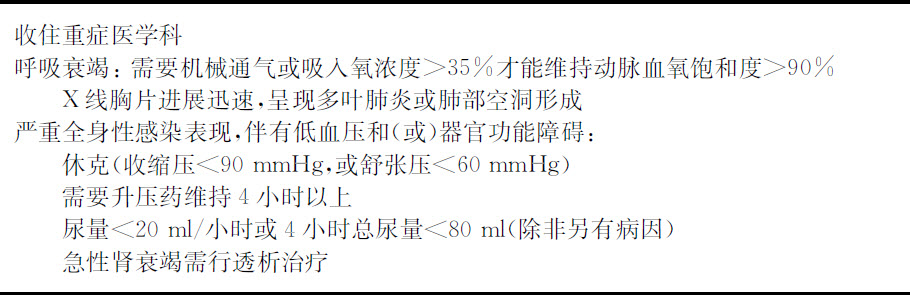
\includegraphics{./images/Image00064.jpg}
\end{table}

\subsection{治疗与预防}

\subsubsection{什么叫合适抗生素治疗?}

2005年美国胸科协会和美国感染病协会制定的医院获得性肺炎和呼吸机相关性肺炎防治指南中,对合适(adequate)抗生素治疗做出了新的定义。对于明确的感染,在进行抗感染治疗时,适当治疗应包括以下4个方面:①选择正确抗生素,即病原菌敏感的抗生素;②使用最佳的抗生素剂量和疗程;③给药途径正确,确保药物渗透到感染部位;④必要时联合用药。只有同时满足上述4个条件,相应的抗生素治疗才是合适的治疗。

\subsubsection{经验性抗菌药物治疗与呼吸机相关性肺炎患者的预后有何关系?}

临床研究表明,早期正确的抗菌药物治疗能够使呼吸机相关性肺炎患者的病死率下降至少一半。此外,有资料显示,正确抗菌药物治疗是否及时也影响呼吸机相关性肺炎患者的预后。早期(进行纤维支气管镜检查前)即接受正确抗菌药物治疗的呼吸机相关性肺炎患者的病死率最低,对于那些使用了错误的经验性治疗的患者,即使后期根据微生物学资料对药物进行调整,也不能降低患者的病死率(分别为71%、70%)。Iregui等研究提示,即使在达到呼吸机相关性肺炎诊断标准后仅延迟合理应用抗菌药物16小时,病死率仍然增加40%。

由于呼吸机相关性肺炎的诊断非常困难,因此在临床高度怀疑呼吸机相关性肺炎时,立即开始正确的经验性抗菌药物治疗就显得非常关键。此外,经验性选择抗菌药物时,需要考虑到患者的基础情况、宿主因素(疾病的严重程度和并发症)、住院时间、既往抗菌药物应用情况、医院或重症医学科中细菌耐药现状等诸多因素,必要时通过联合用药以力求覆盖所有可能的病原体。

因此,及时正确应用抗菌药物是治疗呼吸机相关性肺炎的基石,初始经验性抗菌药物的选择非常重要,因其可以影响患者预后。

\subsubsection{治疗呼吸机相关性肺炎应如何经验性选择抗菌药物?}

2005年美国胸科协会/美国感染病协会制定的医院获得性肺炎和呼吸机相关性肺炎防治指南中,主要根据发病时间的早晚和是否存在多药耐药危险因素决定初始经验性抗菌药物的选择(表\ref{tab8-6}~表\ref{tab8-8})。

\begin{table}[htbp]
{\centering
\caption{已知危险因素且无多药耐药的早发性医院获得性肺炎和呼吸机相关性肺炎患者的初始经验性抗菌药物治疗}
\label{tab8-6}
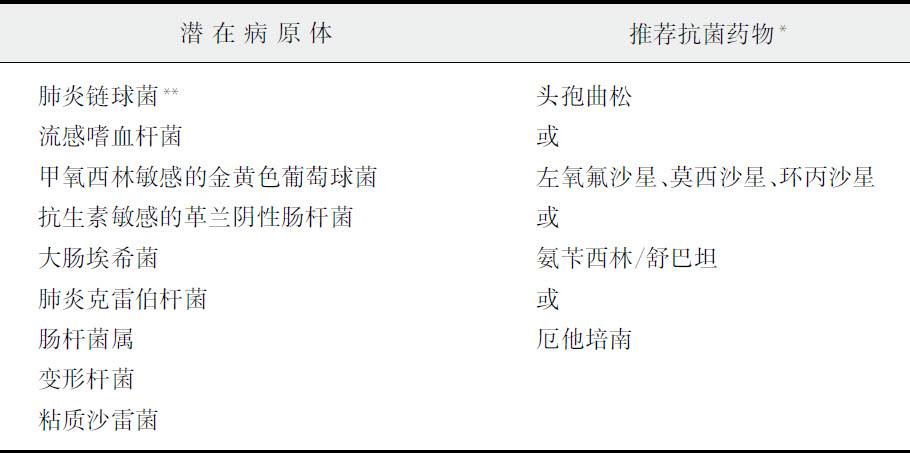
\includegraphics{./images/Image00065.jpg}}

\footnotesize 
* 参照表\ref{tab8-8}选择合适的初始剂量。

**
青霉素耐药的肺炎链球菌和多药耐药的肺炎链球菌在不断增加;左氧氟沙星和莫西沙星优于环丙沙星,其他新型喹诺酮如加替沙星的地位尚不明确。
\end{table}



\begin{table}[htbp]
{\centering
\caption{存在多药耐药危险因素的晚发性重症医院获得性肺炎或呼吸机相关性肺炎患者的初始经验性抗菌药物治疗}
\label{tab8-7}
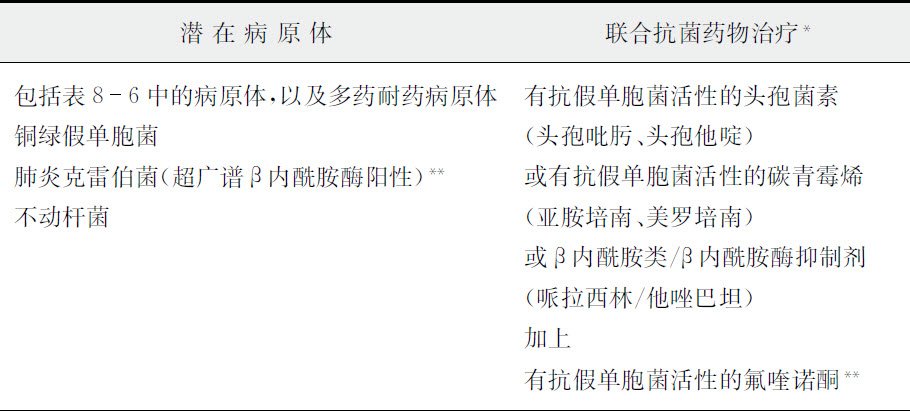
\includegraphics{./images/Image00066.jpg}
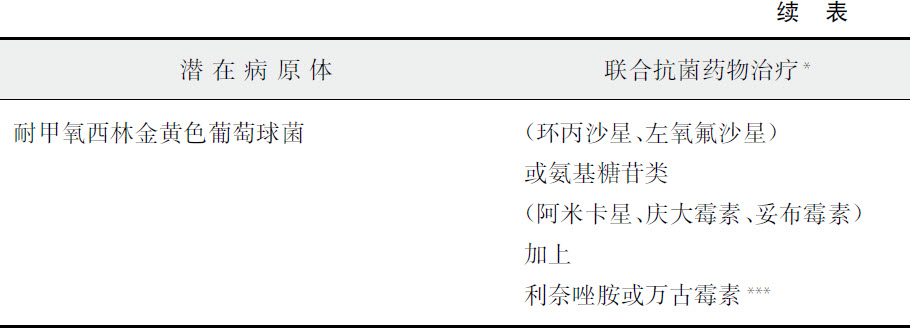
\includegraphics{./images/Image00067.jpg}
}

\footnotesize
*
参照表\ref{tab8-8}选择适当的初始剂量,并根据微生物学结果和临床治疗反应及时调整初期的抗菌药物。

**
如果超广谱β内酰胺酶阳性,且考虑可能是肺炎克雷伯杆菌或不动杆菌感染,碳青霉烯是个可信赖的选择;如果考虑存在嗜肺军团菌感染可能,联合使用一种大环内酯类(如阿奇霉素)或氟喹诺酮类药物(如环丙沙星、左氧氟沙星)治疗优于使用氨基糖苷类。

***
如果存在耐甲氧西林金黄色葡萄球菌危险因素或耐甲氧西林金黄色葡萄球菌在当地有很高的发病率,应联合使用。
\end{table}





\begin{table}[htbp]
\centering
\caption{晚发性或多药耐药病原菌引起的医院获得性肺炎、呼吸机相关性肺炎、卫生保健相关性肺炎的初始经验性抗菌药物的成人静脉给药剂量}
\label{tab8-8}
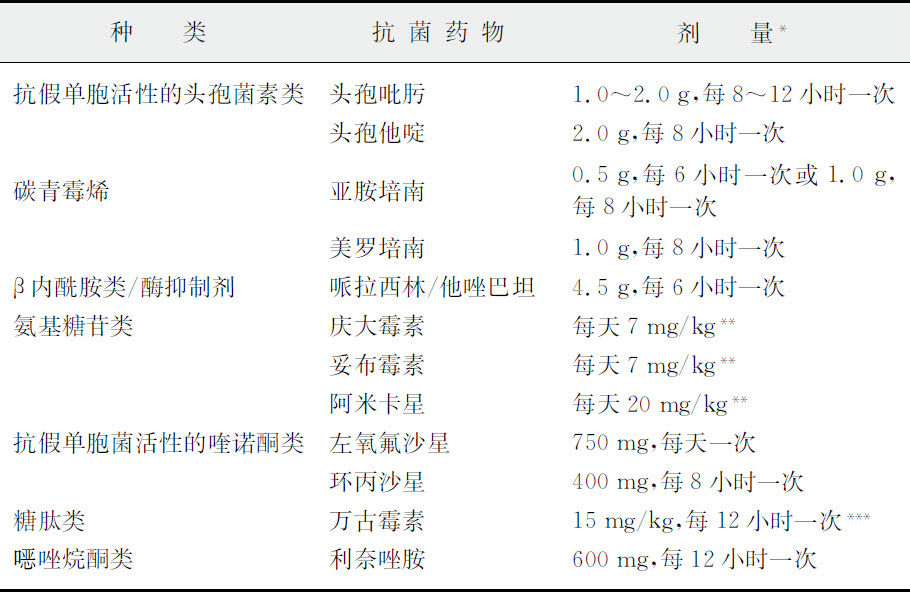
\includegraphics{./images/Image00068.jpg}
\end{table}

* 推荐的剂量是基于正常的肝肾功能。

**
庆大霉素和妥布霉素的谷浓度应低于1μg/ml,阿米卡星的谷浓度应低于4~5μg/ml。

*** 万古霉素的谷浓度在15~20μg/ml。

\subsubsection{如何评价抗菌药物的联合用药在呼吸机相关性肺炎治疗中的意义?}

与单一用药相比,联合用药具有以下优点:①防止耐药细菌的产生;②药物之间可能具有协同和相加作用。

通常,当治疗耐药细菌(如铜绿假单胞菌、多药耐药的不动杆菌、肠杆菌和沙雷菌)引起的严重感染时,需要联合用药。常见的联合用药包括:①氨基糖苷类和β内酰胺类;②氨基糖苷类和喹诺酮类;③喹诺酮类和β内酰胺类。但实际上目前支持联合用药的研究很少。抗菌药物治疗假单胞菌感染的协同作用仅表现在体外试验中,临床治疗也仅能改善中性粒细胞减少和菌血症患者的预后,而这在呼吸机相关性肺炎中并不常见。一项大样本荟萃分析(选择前瞻性随机研究)比较联合β内酰胺类和氨基糖苷类与单用β内酰胺类治疗严重全身感染患者(7586例患者中1200例呼吸机相关性肺炎),结果显示联合用药治疗铜绿假单胞菌感染无任何优势,进一步分析表明联合用药同样不能预防耐药发生,反而使肾毒性明显增加。由此可见对明确的致病菌,联合用药的利弊尚需更多的临床资料去进一步证实。

联合用药目前更多用于初始经验性选择抗菌药物时,为覆盖多药耐药病原菌和可能的混合感染菌的需要。由于联合用药价格昂贵,且让患者暴露于许多不必要的抗菌药物中,有可能导致多药耐药病原菌的发生和不良的预后,因此应尽早明确病原菌,并结合治疗的反应,如有可能应尽早停用不必要的药物(如对治疗临床反应好的患者氨基糖苷类治疗5~7天后停用),或改为单药治疗。对于无多药耐药危险性的、早发性的呼吸机相关性肺炎应首选合适的抗菌药物单一治疗。

\subsubsection{治疗鲍曼不动杆菌感染的常用抗菌药物有哪些?}

(1)舒巴坦及含舒巴坦的β内酰胺类抗生素的复合制剂 舒巴坦对不动杆菌属细菌具抗菌作用,故含舒巴坦的复合制剂对不动杆菌具良好的抗菌活性。对于一般感染,舒巴坦的常用剂量不超过4.0g/天,而多重耐药菌所致感染,国外推荐剂量可增加至6.0g/天,分3~4次给药。肾功能减退患者须调整给药剂量。

(2)碳青霉烯类抗生素 可用于敏感菌所致的各类感染,或与其他药物联合治疗多重耐药菌所致感染。亚胺培南和美罗培南的剂量常需1.0g,每8小时一次或1.0g,每6小时一次,静脉滴注。药代动力学研究显示,对于一些敏感性下降的菌株(最低抑菌浓度4~16mg/L),通过增加给药次数、加大给药剂量、延长静脉滴注时间(如每次静滴时间延长至2~3小时),可使血药浓度高于最低抑菌浓度的时间延长,部分感染病例有效,但目前尚缺乏大规模临床研究。

(3)多黏菌素类抗生素 分为多黏菌素B及多黏菌素E(colistin,粘菌素),临床应用的多为多黏菌素E。国际上推荐多黏菌素E的剂量为每天2.5~5mg/kg或每天200万~400万U(100万U相当于多黏菌素E甲磺酸盐80mg),分2~4次静脉滴注。该类药物的肾毒性及神经系统不良反应发生率高,对于老年人、肾功能不全患者特别需要注意肾功能的监测。另外,多黏菌素E存在明显的异质性耐药,常需联合应用其他抗菌药物。

(4)替加环素(tigecycline) 为甘氨酰环素类抗菌药物,甘氨酰环素类为四环素类抗菌药物米诺环素的衍生物。早期研究发现其对全球分离的碳青霉烯类抗生素耐药鲍曼不动杆菌的最低抑菌浓度\textsubscript{90}
为2mg/L。近期各地报告的敏感性差异大,耐药菌株呈增加趋势,常需根据药敏结果选用。由于其组织分布广泛,血药浓度、脑脊液浓度低,常需与其他抗菌药物联合应用。美国FDA批准该药的适应证为复杂性腹腔及皮肤软组织感染、社区获得性肺炎。常用给药方案为首剂100mg,之后50mg每12小时一次静脉滴注。主要不良反应为胃肠道反应。

(5)四环素类抗菌药物 美国FDA批准米诺环素针剂用于敏感鲍曼不动杆菌感染的治疗,给药方案为米诺环素100mg,每12小时一次静脉滴注,但临床研究不多。国内目前无米诺环素针剂,可使用口服片剂或多西环素针剂(100mg,每12小时一次)与其他抗菌药物联合治疗鲍曼不动杆菌感染。

(6)氨基糖苷类抗生素 这类药物多与其他抗菌药物联合治疗敏感鲍曼不动杆菌感染。国外推荐剂量阿米卡星或异帕米星每天15~20mg/kg,国内常用0.6g每天一次静脉滴注给药,对于严重感染且肾功能正常者,可加量至0.8g/天给药。用药期间应监测肾功能及尿常规,最好监测血药浓度。

(7)其他 对鲍曼不动杆菌具抗菌活性的其他抗菌药物尚有喹诺酮类抗菌药物、第三及第四代头孢菌素如头孢他啶、头孢吡肟,其他β内酰胺酶抑制剂的复合制剂如哌拉西林/他唑巴坦,但耐药率高,达64.1%~68.3%,故应根据药敏结果选用。体外及动物体内研究显示,利福平与其他抗菌药联合对不动杆菌有协同杀菌作用,因其为治疗结核病的主要药物之一,不推荐常规用于鲍曼不动杆菌感染的治疗。

\subsubsection{如何合理选择抗菌药物治疗鲍曼不动杆菌感染?}

(1)非多重耐药鲍曼不动杆菌感染 可根据药敏结果选用β内酰胺类抗生素等抗菌药物。

(2)多重耐药鲍曼不动杆菌感染 根据药敏选用头孢哌酮/舒巴坦、氨苄西林/舒巴坦或碳青霉烯类抗生素,可联合应用氨基糖苷类抗生素或氟喹诺酮类抗菌药物等.

(3)广泛耐药鲍曼不动杆菌感染 常采用两药联合方案,甚至三药联合方案。两药联合用药方案有------①以舒巴坦或含舒巴坦的复合制剂为基础的联合,联合以下一种:米诺环素(或多西环素)、多黏菌素E、氨基糖苷类抗生素、碳青霉烯类抗生素等;②以多黏菌素E为基础的联合,联合以下一种:含舒巴坦的复合制剂(或舒巴坦)、碳青霉烯类抗生素;③以替加环素为基础的联合,联合以下一种:含舒巴坦的复合制剂(或舒巴坦)、碳青霉烯类抗生素、多黏菌素E、喹诺酮类抗菌药物、氨基糖苷类抗生素。三药联合方案有:含舒巴坦的复合制剂(或舒巴坦)+多西环素+碳青霉烯类抗生素、亚胺培南+利福平+多黏菌素或妥布霉素等。

(4)全耐药鲍曼不动杆菌感染 常需通过联合药敏试验筛选有效的抗菌药物联合治疗方案。研究发现,鲍曼不动杆菌易对多黏菌素产生异质性耐药,但异质性耐药菌株可部分恢复对其他抗菌药物的敏感性,因此多黏菌素联合β内酰胺类抗生素或替加环素是可供选择的方案,但尚缺少大规模临床研究。也可结合抗菌药物药代动力学参数要求,尝试通过增加给药剂量、增加给药次数、延长给药时间等方法设计给药方案。

\subsubsection{控制导管生物被膜对防治呼吸机相关性肺炎有何意义?}

细菌生物被膜(biofilm,BF)指细菌粘附于固体或有机腔道表面,形成微菌落,并分泌多糖蛋白复合物将自身包裹其中而形成的膜状物。目前认为细菌BF是导致某些慢性感染反复发作难以治愈的重要原因。其机制包括:①阻滞抗菌药物的渗透;②吸附抗菌药物灭活酶,促进抗菌药物水解;③被膜下细菌代谢低下,呈“亚冬眠状态”,对抗菌药物敏感性低;④阻滞机体免疫系统对细菌的清除,产生免疫逃逸现象,减弱机体免疫力与抗菌药物的协同杀菌作用。临床上容易形成生物被膜的致病菌主要有铜绿假单胞菌、金黄色葡萄球菌、表皮葡萄球菌、大肠埃希菌等。

有研究表明,气管导管表面的细菌生物被膜是导致呼吸机相关性肺炎发生和病情反复的重要原因之一,临床应创造条件尽早拔除气管导管,以减少导管内外细菌生物被膜的形成。国外有人从事抗定植材料的研究,但目前由这种材料制成的导管尚未面世。有报道氟喹诺酮类和大环内酯类(14-元环或者5-元环)抗菌药物可抑制细菌生物被膜的形成,并破坏已形成的细菌生物被膜。

\subsubsection{呼吸机相关性肺炎的非抗生素防治措施有哪些?}

呼吸机相关性肺炎的发生增加患者的住院时间、费用,病死率也明显增加。在抗菌药物抗感染的同时,我们更需关注非抗生素的抗感染防治措施,这有时比抗菌药物更为重要,尤其在病原体为多药耐药或泛耐药的时候。而且实施以下防治策略时应建议采取综合性、集束化(bundle)的非抗生素策略,其主要措施有------①一般性措施,包括手部清洁,戴手套和穿隔离衣,洗必泰口腔护理;②与消化道相关控制策略包括合适的应激性溃疡预防,避免胃过度扩张,避免长时间留置经鼻胃管,应用较细的营养管路,早期的胃造瘘和应用空肠营养;③与患者体位相关策略:保持半卧位(30°~45°),应用动力翻身床,不常规推荐俯卧位;④与人工气道相关策略:避免经鼻气管插管,维持合适的气囊压力(20cm
H\textsubscript{2} O以上,一般25~35cm H\textsubscript{2}
O)和持续声门下吸引;⑤机械通气相关策略:定期的呼吸机设备的清洁,避免不必要频繁更换呼吸机管路,避免过度镇静,每日间断唤醒,减少机械通气时间和尽早脱机;⑥其他措施:合适的血糖控制,控制在8.3mmol/L以下,限制制酸药的使用,增强患者免疫功能。

\subsubsection{如何评价洗必泰口腔护理对于呼吸机相关性肺炎防治的意义?}

在口腔和牙菌斑积聚的细菌进入下呼吸道是导致呼吸机相关性肺炎的重要原因。洗必泰溶液可以控制牙菌斑上细菌生长。临床研究表明,与常规口腔护理相比,对心脏外科术后患者用洗必泰漱口,实施口咽部去污染,可使医院获得性感染的发生率从13.3%降低到4.6%(\emph{P}
<0.01),治疗性抗生素应用也明显降低(23.3%对比13.3%,\emph{P}
<0.05)。更值得注意的是,洗必泰漱口去污染组患者的病死率为1.16%,明显低于常规口腔护理组(5.56%,\emph{P}
<0.05)
\protect\hyperlink{text00014.htmlux5cux23ch7-13}{\textsuperscript{{[}7{]}}}
。另外,实施洗必泰口咽部去污染对抗生素耐药致病菌的局部定植也有明显预防作用。

洗必泰口腔护理简单可行、费用不高,对高危患者应常规使用。

\subsubsection{机械通气患者如何进行应激性溃疡的预防?}

一般认为,危重患者特别是机械通气患者,是上消化道出血的危险人群,应用抑酸药(H\textsubscript{2}
受体阻滞剂或质子泵抑制剂)提高胃液pH值成为预防上消化道出血的常用措施。但胃是口咽部革兰阴性定植菌的主要来源。健康人胃内pH低于2,基本处于无菌状态。但当胃内pH高于4时,微生物即在胃内大量繁殖。研究表明,当pH增加到6.0时,胃液内菌落可增至10\textsuperscript{7}
cfu/ml以上,成为细菌侵入下呼吸道的潜在感染源。因此,避免使用抑酸药,避免胃液pH值的升高,将有助于预防呼吸机相关性肺炎。而硫糖铝口服或鼻饲后,对胃黏膜具有保护作用,能够预防上消化道出血的发生,同时硫糖铝对胃液pH值无明显影响,已有研究显示,与H\textsubscript{2}
受体阻滞剂相比可以降低呼吸机相关性肺炎的发生率。

近年多中心随机双盲对照研究(\emph{n}
=1200)显示,危重病患者应用H\textsubscript{2}
受体拮抗剂雷尼替丁预防应激性溃疡,危及生命的上消化道出血发生率为1.7%;胃黏膜保护剂硫糖铝组发生率为3.8%,H\textsubscript{2}
受体拮抗剂明显优于硫糖铝,但两组呼吸机相关性肺炎发生率分别为19.1%和16.2%,无统计学差异。

因此,对于出血倾向小的患者可建议常规应用硫糖铝进行应激性溃疡的预防;当存在危及生命的上消化道出血风险时则不推荐单独应用硫糖铝,可使用抑酸药预防应激性溃疡。

\subsubsection{如何评价热湿交换器与加温湿化器在呼吸机相关性肺炎防治中的意义?}

人工气道的湿化非常重要,目前临床上常用的湿化装置有加温湿化器(heated
humidifier)和热湿交换器(heated moisture exchanger)。Dedek等
\protect\hyperlink{text00014.htmlux5cux23ch3-13}{\textsuperscript{{[}3{]}}}
在基于循证医学的呼吸机相关性肺炎预防指南中指出:对于无禁忌证(如咯血或高分钟通气量通气)的患者推荐使用热湿交换器进行湿化,并建议每周更换热湿交换器。而2005年美国胸科协会和美国感染病协会关于院内获得性肺炎和呼吸机相关性肺炎指南中建议的不同,即被动式加湿器或热湿交换器能减少呼吸机管路的细菌定植,但并未减少呼吸机相关性肺炎的发生率,因此不能将其作为肺炎的预防措施。近期研究也显示热湿交换器并不降低呼吸机相关性肺炎的发生率,且在Lorente等
\protect\hyperlink{text00014.htmlux5cux23ch10-13}{\textsuperscript{{[}10{]}}}
对104例机械通气患者随机对照研究中发现,机械通气5天以上,患者使用加温湿化器的呼吸机相关性肺炎发生率低于热湿交换器,回归分析显示热湿交换器是呼吸机相关性肺炎的独立危险因素。

因此,目前不建议使用热湿交换器防治呼吸机相关性肺炎,但鉴于其使用方便,在无禁忌证的情况下可用于短期机械通气患者的湿化。

\subsubsection{如何评价无创通气在呼吸机相关性肺炎防治中的意义?}

无创通气可以避免气管插管和气管切开引起的并发症,保留了上呼吸道的防御能力。对于部分合并免疫抑制的急性肺损伤和急性呼吸窘迫综合征患者,使用无创通气有助于避免呼吸机相关性肺炎的发生。另有部分研究显示,与有创机械通气相比,给予无创通气治疗,可明显减少抗生素用量、缩短重症医学科住院时间,并最终能够降低患者的病死率。目前认为,对于慢性阻塞性肺疾病急性加重期、急性呼吸衰竭早期、急性心源性肺水肿和免疫功能低下的患者,如无禁忌可首先考虑无创通气。但是,对于重症急性呼衰患者,无创通气既不降低插管率,也不改善预后,甚至可能由于气道没有保障而加重病情。因此,把握无创通气的应用指征和转为有创通气的时机非常重要。

\begin{center}\rule{0.5\linewidth}{\linethickness}\end{center}

参考文献

\protect\hyperlink{text00014.htmlux5cux23ch1-13-back}{{[}1{]}}
.American Thoracic Society Documents:Guidelines for the management of
adults with hospital-acquired,ventilator-associated,and
healthcare-associated pneumonia.Am J Respir Crit Care
Med,2005,171:388-416.

\protect\hyperlink{text00014.htmlux5cux23ch2-13-back}{{[}2{]}}
.Dellinger RP,Carlet JM,Masur H,et al.Surviving Sepsis Campaign
guidelines for management of severe sepsis and septic shock.Crit Care
Med,2004,32:858-873.

\protect\hyperlink{text00014.htmlux5cux23ch3-13-back}{{[}3{]}} .Dodek
P,Keenan S,Cook D,et al.Evidence-based clinical practice guideline
for the prevention of ventilator-associated pneumonia.Ann Intern
Med,2004,141:305-313.

\protect\hyperlink{text00014.htmlux5cux23ch4-13-back}{{[}4{]}}
.Porzecanski I,Bowton DL.Diagnosis and treatment of
ventilator-associated pneumonia.Chest,2006,130:597-604.

\protect\hyperlink{text00014.htmlux5cux23ch5-13-back}{{[}5{]}}
.Gujadhur R,Helme BW,Sanni A,et al.Continuous subglottic suction is
effective for prevention of ventilator-associated pneumonia.Interact
Cardio Vasc Thorac Surg,2005,4:110-115.

\protect\hyperlink{text00014.htmlux5cux23ch6-13-back}{{[}6{]}}
.Kostadima E,Kaditis G,Alexopoulos I,et al.Early gastrostomy
reduces the rate of ventilator-associated pneumonia in stroke or head
injury patients.Eur Respir J,2005,26:106-111.

\protect\hyperlink{text00014.htmlux5cux23ch7-13-back}{{[}7{]}} .Koeman
M,van der Ven AJAM,Hak E,et al.Oral decontamination with
chlorhexidine reduces the incidence of ventilator-associated
pneumonia.Am J Respir Crit Care Med,2006,173:1348-1355.

\protect\hyperlink{text00014.htmlux5cux23ch8-13-back}{{[}8{]}} .Macleod
R,Bucknall T.Mechanical ventilation with heated humidifiers or with
heat and moisture exchangers with microbiological filters did not reduce
ventilator associated pneumonia in adults.Evid Based
Nurs,2006,9:82.

{[}9{]}.Lacherade JC,Auburtin M,Cerf C,et al.Impact of
humidification systems on ventilator-associated pneumonia:A randomized
multicenter trial.Am J Respir Crit Care Med,2005,172:1276-1282.

\protect\hyperlink{text00014.htmlux5cux23ch10-13-back}{{[}10{]}}
.Lorente L,lecuona M,Jimenez A,et al.Ventilator-associated
pneumonia using a heated humidifier or a heat and moisture exchanger:a
randomized controlled trial.Crit Care,2006,10:R116.

\protect\hyperlink{text00014.htmlux5cux23ch11-13-back}{{[}11{]}}
.Fujitani S,Aspirates E,Shigeki,et al. Diagnosis of
ventilator-associated pneumonia:focus on nonbronchoscopic
techniques(nonbronchoscopic bronchoalveolar lavage,including
mini-BAL,blinded protected specimen brush,and blinded bronchial
sampling)and endotracheal aspirates.J Intensive Care
Med,2006,21:17-21.

\protect\hyperlink{text00014.htmlux5cux23ch12-13-back}{{[}12{]}} .Luna
C,Niederman MS,Baredes NC,et al.Resolution of ventilator-associated
pneumonia:prospective evaluation of the clinical pulmonary infection
score as an early clinical predictor of outcome.Crit Care
Med,2003,31:676-682.

\protect\hyperlink{text00014.htmlux5cux23ch13-13-back}{{[}13{]}}
.Khaleeq G,Garcha P,Hirani A,et al.Clinical pulmonary infection
score(CPIS)relationship to mortality in patients with ventilator
associated pneumonia.Chest Meeting Abstracts,2006,130:218S-219S.

\protect\hypertarget{text00015.html}{}{}

